    \section{Μετασχηματισμός Laplace}
    \begin{align*}
        \nexists\, X(\omega ) &= \int_{-\infty}^{\infty} x(t)e^{-j\omega t}\dif t\\
        y(t) &= x(t)e^{-\sigma t}\\
        \exists\, Y(\omega ) &= \int_{-\infty}^{\infty} y(t)e^{-j\omega t}\dif t
        \quad (s=\sigma+j\omega ) \\ &= \int_{-\infty}^{\infty} x(t)
        e^{-\sigma t}e^{-j\omega t}\dif t \\
        \Aboxed{ X(s) &= \int_{-\infty}^{\infty} x(t)e^{-st}\dif t }
        \quad \text{Μ. Laplace}
    \end{align*}
    
    \paragraph{Αντίστροφος μετασχηματισμός Laplace}
    \( \displaystyle
    x(t) = \frac{1}{2\pi j}
    \int_{\sigma-j\underset{\mathclap{(-\infty)}}{\omega} }^{
        \sigma+j\overset{\mathclap{(\infty)}}{\omega}} X(s)e^{st}\dif s
     \)
     
     \paragraph{}
     
    \begin{itemize}
        \item Έστω ότι \( x(t) \) είναι αιτιατή (\( x(t)=0 \quad t< 0 \)).
        
        Ας φανταστούμε ότι η \( x(t) \) δεν έχει μετασχηματισμό Fourier.
        
        \begin{tikzpicture}[scale=1,xscale=1]
        \fill[samples=30,domain=0:4,smooth,variable=\x,blue!10] 
        plot ({\x},{exp(\x/2-1)}) -- (4,0) -- (0,0) -- cycle;
        \fill[samples=30,domain=0:4,smooth,variable=\x,blue!10] 
        plot ({\x},{-exp(\x/2-1)}) -- (4,0) -- (0,0) -- cycle;
        
        \draw[->] (0,-2) -- (0,2); %node[right] {$f(t)$};
        \draw[->] (-2,0) -- (4,0) node[below,right] {$t$};
        
        \draw[samples=100,domain=4:0,smooth,variable=\x,blue,very thick] 
        plot ({\x},{-exp(\x/2-1)* sin(-5*\x r)});
        \draw[samples=50,domain=4:0,smooth,variable=\x,blue] 
        plot ({\x},{exp(\x/2-1)}) plot ({\x},{-exp(\x/2-1)});
        
        \draw (0,-2) node[below] {$x(t) = \sin( \omega t)\, e^t \mathrm u(t)$};
        
        \begin{scope}[xshift=7cm]
        \fill[green!70] (1,-2) rectangle (0.7,2);
        \fill[green!70,path fading=east] (2,-2) rectangle (1,2);
        
        \draw[->] (-2,0) -- (2,0) node[below] {$\sigma$};
        \draw[->] (0,-2) -- (0,2) node[right] {$j\omega$};
        
        \draw[dashed] (0.7,-2) -- ++(0,4);
        \draw (0.7,0) node[above left] {$1$};
        
        \draw (-1,-1) node {$s$-plane};
        \draw (2,-1) node {$\Re\lbrace s\rbrace = \sigma>1$};
        \end{scope}
        \end{tikzpicture}
        
        \vspace{5pt}
        
        \begin{tikzpicture}[scale=1,xscale=1]
        \fill[samples=30,domain=0:4,smooth,variable=\x,blue!10] 
        plot ({\x},{exp(-\x/1.5+0.5)}) -- (4,0) -- (0,0) -- cycle;
        \fill[samples=30,domain=0:4,smooth,variable=\x,blue!10] 
        plot ({\x},{-exp(-\x/1.5+0.5)}) -- (4,0) -- (0,0) -- cycle;
        
        \draw[->] (0,-2) -- (0,2); %node[right] {$f(t)$};
        \draw[->] (-2,0) -- (4,0) node[below,right] {$t$};
        
        \draw[samples=100,domain=4:0,smooth,variable=\x,blue,very thick] 
        plot ({\x},{-exp(-\x/1.5+0.5)* sin(-5*\x r)});
        \draw[samples=50,domain=4:0,smooth,variable=\x,blue] 
        plot ({\x},{exp(-\x/1.5+0.5)}) plot ({\x},{-exp(-\x/1.5+0.5)});
        
        \draw (0,-2) node[below] {$x(t) = \sin( \omega t)\, e^{-t} \mathrm u(t)$};
        
        \begin{scope}[xshift=7cm]
        \fill[green!70] (-0.3,-2) rectangle (-0.7,2);
        \fill[green!70,path fading=east] (-0.3,-2) rectangle (2,2);
        
        \draw[->] (-2,0) -- (2,0) node[below] {$\sigma$};
        \draw (0,-2) -- (0,2);
        
        \draw[dashed] (-0.7,-2) -- ++(0,4);
        \draw (-0.7,0) node[above left] {$-1$};
        
        \draw (2,-1) node {$\Re\lbrace s\rbrace = \sigma>-1$};
        \end{scope}
        \end{tikzpicture}
        
        \item Έστω ότι \( x(t) \) αντιαιτιατή (\( x(t)=0 \quad t>0 \))
        
        \begin{tikzpicture}[scale=1,xscale=1]
        
        \fill[samples=30,domain=-4:0,smooth,variable=\x,blue!10] 
        plot ({\x},{exp(-\x/2-1)}) -- (0,0) -- (-4,0) -- cycle;
        \fill[samples=30,domain=-4:0,smooth,variable=\x,blue!10] 
        plot ({\x},{-exp(-\x/2-1)}) -- (0,0) -- (-4,0) -- cycle;
        
        \draw[->] (0,-2) -- (0,2); %node[right] {$f(t)$};
        \draw[->] (-4,0) -- (3,0) node[below,right] {$t$};
        
        \draw[samples=100,domain=-4:0,smooth,variable=\x,blue,very thick] 
        plot ({\x},{-exp(-\x/2-1)* sin(5*\x r)});
        \draw[samples=50,domain=-4:0,smooth,variable=\x,blue] 
        plot ({\x},{exp(-\x/2-1)}) plot ({\x},{-exp(-\x/2-1)});
        
        \draw (0,-2) node[below] {$x(t) = \sin \omega t\, e^{-t} \mathrm u(-t)$};
        
        \begin{scope}[xshift=6cm]
        \fill[green!70] (-1,-2) rectangle (-0.7,2);
        \fill[green!70,path fading=west] (-2,-2) rectangle (-1,2);
        
        \draw[->] (-2,0) -- (2,0);
        \draw (0,-2) -- (0,2);
        
        \draw[dashed] (-0.7,-2) -- ++(0,4);
        \draw (-0.7,0) node[above right] {$-1$};
        
        \draw (1,1) node {$s$-plane};
        \end{scope}
        \end{tikzpicture}

        
        \item \mbox{}
        \\
        \begin{tikzpicture}[scale=1,xscale=0.5]
        
        \fill[green!70,path fading=east] (0,-2) rectangle (5,2) ;
        
        \draw (-2,0) -- (4,0);
        \draw (0,-2) -- (0,2);
        
        \draw (0,0) node[below left] {$\mathsmaller{0}$};
        
        \draw (0,-2) node[below right] {$\Re \lbrace s \rbrace \geq 0 $};
        
        \begin{scope}[xshift=9cm]
        \fill[green!50!blue!70!white,path fading=west] (1,-2) rectangle (-3,2) ;
        
        \draw (-2,0) -- (4,0);
        \draw (0,-2) -- (0,2);
        
        \draw (1,0) node[below right] {$1$};
        
        \draw (0,-2) node[below right] {$\Re \lbrace s \rbrace < 1$};
        \draw[dashed] (1,-2) -- ++(0,4);
        \end{scope}
        
        \begin{scope}[xshift=16cm]
        \fill[green!70!blue!50!white] (1,-2) rectangle (0,2) ;
        
        \draw (-2,0) -- (4,0);
        \draw (0,-2) -- (0,2);
        
        \draw (1,0) node[below right] {$1$};
        \draw[dashed] (1,-2) -- ++(0,4);
        \end{scope}
        
        \draw (current bounding box.north west) node[above right]
        {$\sin \omega t\, \mathrm u(t) + \sin \omega t\, e^t \mathrm u(-t)$};
        \end{tikzpicture}
        
        \item Η \( \sin \omega \mathrm u(t)+\sin\omega t e^{-t}\mathrm u(-t) \)
        δεν έχει περιοχή σύγκλισης.
    \end{itemize}
    
    \[
    X(s) = \frac{35}{(x-8)(x+2)}
    \]
    
    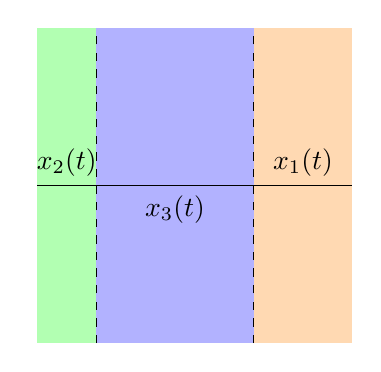
\begin{tikzpicture}[scale=1,xscale=0.5]
    
    \fill[green!30] (-4,-2) rectangle (-2.5,2) node[black,pos=.5,above] {$x_2(t)$};
    \fill[blue!30] (-2.5,-2) rectangle (1.5,2) node[black,pos=.5,below] {$x_3(t)$};
    \fill[orange!30] (1.5,-2) rectangle (4,2) node[black,pos=.5,above] {$x_1(t)$};
    
    \draw (-4,0) -- (4,0);
    \draw [dashed](-2.5,-2) -- ++(0,4);
    \draw[dashed] (1.5,-2) -- ++(0,4);
    \end{tikzpicture}
    
    Οι πόλοι (ρίζες του παρονομαστή) καθορίζουν τις περιοχές σύγκλισης.
    
    \paragraph{}
    Οι συναρτήσεις που χρησιμοποιούμε είναι αιτιατές, άρα γενικά ο μετασχηματισμός
    Laplace καταρρέει στην:
    \[
    X(s) = \int_{0^-}^{\infty} x(t)e^{-st}\dif t
    \]
    
    Το \( 0^- \) μάς επιτρέπει να ασχοληθούμε με συναρτήσεις που απειρίζονται
    στο 0, π.χ. \( \frac{1}{x} \) or \( \delta(t) \).
    
    \subsection{Ιδιότητες}
    \( x(t)\to X(s) \quad \Re\left\lbrace s \right\rbrace > \sigma_1 \)
    
    \( y(t)\to\, Y(s) \quad \Re\left\lbrace s \right\rbrace > \sigma_2 \)
    
    \begin{enumpar}
    \item \(\displaystyle ax(t)+by(t) \to aX(s)+bY(s) \qquad \text{τουλάχιστον }
    \Re\left\lbrace s \right\rbrace >
     \max\left\lbrace \sigma_1,\sigma_2 \right\rbrace\)
     \item Μετατόπιση σε χρόνο
    \begin{align*}
    x(t)\mathrm u(t)\to X(s)\quad & \sigma>\sigma_1 \\
    y(t) = x(t-t_0)\mathrm u(t-t_0)\to X(s)e^{-t_0s} 
    \quad & t_0>0 \quad \sigma>\sigma_2
    \end{align*}
    \subparagraph{Απόδ.}
    \begin{align*}
    Y(s) = \int_{0^-}^\infty y(t)e^{-st}\dif t
    = \int_{0^-}^{\infty} x(\underbrace{t-t_0}_{\tau})\mathrm u(t-t_0)e^{-st}\dif t
    = x(\tau)\mathrm u(\tau)e^{-s(t+t_0)}\dif\tau = X(s)e^{-st_0}
    \end{align*}
    \item Κλιμάκωση
    \begin{gather*}
    x(t)\to X(s) \\
    x(at)\to\frac{1}{a}X\left(\frac{s}{a}\right)\quad a>0
    \end{gather*}
    \item Παραγώγιση
    \begin{gather*}
    x(t)\to X(s) \\
    \od{x(t)}{t}\to sX(s)-x\left(0^- \right)
    \end{gather*}
    \item Ολοκλήρωση
    \begin{gather*}
    x(t)\to X(s) \\
    \int_0^t x(t)\dif t \to \frac{1}{s}X(s)
    \end{gather*}
    \item Διαμόρφωση
    \begin{align*}
    x(t)\to X(s) &\qquad \sigma>\sigma_1 \\
    e^{-at}x(t)\to X(s+a) &\qquad 
    a\in\mathbb C \qquad \sigma>\sigma_1 - \Re\left\lbrace a \right\rbrace
    \end{align*}
    \item Συνέλιξη
    \begin{gather*}
    x(t)\to X(s)\\
    y(t) \to Y(s)
    \end{gather*}
    \[
    x(t)*y(t)=X(s)Y(s)
    \]
    \end{enumpar}
    
    \subsection{Laplace "περιοδικών συναρτήσεων"}
    \[
    x_T(t)=\begin{cases}
    x(t) &\quad 0\leq x \leq T \\
    0 &\quad \text{αλλού}
    \end{cases}
    \]
    
    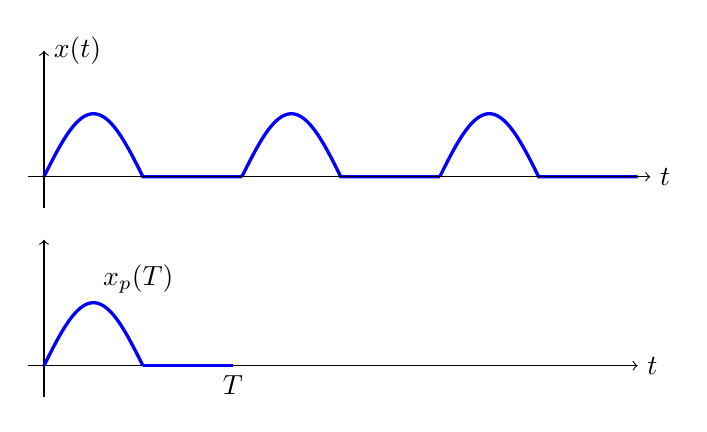
\begin{tikzpicture}[scale=0.8,xscale=0.5]
    
    \begin{scope}
    \draw[->] (0,-0.5) -- (0,2) node[right] {$x(t)$};
    
    \draw[samples=50,domain=0:pi,smooth,variable=\x,blue,very thick] 
    plot ({\x},{sin(\x r)}) -- (2*pi,0);
    \draw[samples=50,domain=2*pi:3*pi,smooth,variable=\x,blue,very thick] 
    plot ({\x},{sin(\x r)}) -- (4*pi,0);
    \draw[samples=50,domain=4*pi:5*pi,smooth,variable=\x,blue,very thick] 
    plot ({\x},{sin(\x r)}) -- (6*pi,0);
    
    \draw[->] (-0.5,0) -- (6*pi+0.4,0) node[below,right] {$t$};
    \end{scope}
    
    \begin{scope}[yshift=-3cm]
    \draw[->] (0,-0.5) -- (0,2); %node[right] {$f(t)$};
    \draw[->] (-0.5,0) -- (6*pi,0) node[below,right] {$t$};
    
    \draw (6,0) node[below] {$T$};
    \draw(pi/2,1) node[above right] {$x_p(T)$};
    
    \draw[very thick, blue] (pi-0.01,0) -- (6,0);
    
    \draw[samples=200,domain=0:pi,smooth,variable=\x,blue,very thick] 
    plot ({\x},{sin(\x r)});
    
    \end{scope}
    
    \end{tikzpicture}
    
    \begin{align*}
    x(t)&=x_T(t)+x_T(t-T)+x_T(t-2T)+\dots\\
    x(t)&= \sum_{n=0}^\infty x_T (t-nT) \\
    \mathscr L\left\lbrace x(t) \right\rbrace &= \sum_{n=0}^\infty
    \mathscr L \left\lbrace x_T(t-uT) \right\rbrace \\[3pt]
    x_T(t) &\xrightarrow{\mathscr L} X^T(s)\\
    x_T(t-nT) &\xrightarrow{\mathscr L} X^T(s)e^{-nTs} \\
    \mathscr L\left\lbrace x(t) \right\rbrace
    &= \sum_{n=0}^\infty X^T(s)e^{-nTs}
    = X^T(s)\sum_{n=0}^\infty e^{-nTs} = \frac{1}{1-e^{-Ts}}X^T(s)
    \quad \sigma>\max(0,\sigma_1)
    \end{align*}
    
    \paragraph{}
    \( \displaystyle X(s) \xrightarrow{?} X(\omega ) \)
    
    \[
    X(\omega ) = \left. X(s)\right|_{s=j\omega }
    \]
    
    \paragraph{Ex. 1}
    \( x(t)= e^{-at}\mathrm ut() \)
    
    \( \displaystyle
    X(s) = \int_{0^-}^\infty x(t)e^{-st}\dif t
    =\int_{0^-}^\infty e^{-at}e^{-st}\dif t
    = \int_{0^-}^\infty e^{-(a+s)t}\dif t
    =\left. \frac{e^{-(a+s)t}}{-(a+s)}\right|_0^\infty
    = \frac{\cancelto{0}{e^{-(a+s)\infty}} -\cancelto{1}{e^{-(a+s)0}} }{-(a+s)}
    = \boxed{\frac{1}{s+a} \quad 
        \Re\left\lbrace s \right\rbrace > \Re\left\lbrace a \right\rbrace}
     \)
     
     
   \paragraph{Ex. 2}
   \( x(t)=\delta(t) \)
   
   \( \displaystyle
   X(t) = \int_{0^-}^\infty \delta(t)e^{-st}\dif t = e^{-s0} = 1 \quad s\in\mathbb C 
    \)
    
   \paragraph{Ex. 3}
   \( x(t)=\mathrm u(t) \qquad X(s)=\frac{1}{s} 
   \quad \Re\left\lbrace s \right\rbrace > 0\)
   
   Για να βρω πεδίο σύγκλισης: \( \displaystyle
   X(s) =
   \int_{0^+}^\infty 1e^{-st}\dif t = \left.
   \frac{e^{-st}}{-s}\right|_{0^-}^\infty
   = \frac{e^{-s\infty}-\cancelto{1}{e^{-s0}}}{-s}=\frac{1}{s}
    \)
    
   \paragraph{Ex. 4}
   \( x(t)=\cos\omega_0 t\, \mathrm u(t) \)
   
   \( \displaystyle
   x(t) = \frac{e^{j\omega_0 t}+e^{-j\omega_0 t}}{2}\, \mathrm u(t)
   =\frac{1}{2}e^{j\omega_0 t}\mathrm u(t)
   +\frac{1}{2}e^{-j\omega_0 t}\mathrm u(t)
   \xrightarrow{\mathscr L \mathrm T}
    \frac{1}{2}
    \underset{\sigma >0}{\frac{1}{s-j\omega_0}}+
    \underset{\sigma >0}{\frac{1}{2}\frac{1}{s+j\omega_0}}
    = \frac{1}{2} \frac{2s}{s^2+\omega_0^2}
    =\frac{s}{s^2+\omega_0^2} \quad \Re\left\lbrace s \right\rbrace>0
    \)
    
    \paragraph{Ex. 5}
    \( x(t)=\sin\omega_0 t\, \mathrm u(t) \)
    
    \( \displaystyle
    \frac{1}{2j}\left[
    e^{j\omega_0 t}\mathrm u(t)-e^{-j\omega_0 t}\mathrm u(t)
    \right] \xrightarrow{\mathscr L \mathrm T}
    \frac{1}{2j}\underset{\Re\left\lbrace s \right\rbrace>0}{
        \left[ \frac{1}{s-j\omega_0} - \frac{1}{s+j\omega_0} \right]
    } = \frac{\omega_0}{s^2+\omega_0^2}
     \qquad \Re \left\lbrace s \right\rbrace > 0
     \)
     
    Ποιός είναι ο μετασχηματισμός Fourier της παραπάνω;
    
    Το πιθανό λάθος αποτέλεσμα είναι το \( 
    \displaystyle \left(
    \xrightarrow[s=j\omega ]{FT} \frac{\omega_0}{\omega_0^2-\omega^2}
    \right)
     \)
     
    \( x(t) = \sin\omega_0t\, \mathrm u(t) \)
    
    \begin{align*}
    \sin\omega_0 t &\xrightarrow{\mathrm{FT}} j\pi\left[
    -\delta(\omega-\omega_0)+\delta(\omega +\omega_0)
    \right] \\
    \mathrm u(t) &\xrightarrow{\mathrm{FT}} \pi\delta(\omega )+\frac{1}{j\omega }
    \end{align*}
    \begin{align*}
    x(t) &\to \left[
    j\pi\left(\delta(\omega +\omega_0)-\delta(\omega -\omega_0) \right)
    \right] * \left[
    \pi\delta(\omega )+\frac{1}{j\omega }
    \right] \\
    &= \frac{1}{2\pi}\left[
    j\pi^2\left(
    \delta(\omega+\omega_0)-\delta(\omega-\omega_0)
    \right) +j\pi\left(
    \frac{1}{j(\omega+\omega_0)}-\frac{1}{j(\omega+\omega_0)}
    \right)    \right]
    \\ &= \frac{j\pi}{2}\left[
    \delta(\omega +\omega_0)-\delta(\omega-\omega_0)\right]+\left[
    \frac{\omega_0}{\omega_0^2-\omega^2}
    \right] 
    \end{align*}
    
    \begin{theorem*}[title=Θεωρήματα Αρχικής \& Τελικής Τιμής,width=.5\textwidth]%
        {Αρχικής \& Τελικής Τιμής}
    \begin{align*}
    \lim_{t\to 0^+} x(t) &= \lim_{s\to \infty} \left( sX(s) \right) \\
    \lim_{t\to \infty} x(t) &= \lim_{s\to 0} \left( sX(s) \right)
    \end{align*}
    \end{theorem*}
    
    \begin{gather*}
    (-t)^n f(t) \xrightarrow{\mathscr L T} \od[n]{F(s)}{s} \\
    f(t) \xrightarrow{\mathscr L T} F(s)
    \end{gather*}
    
    Για να βρίσκουμε αντίστροφους μετασχηματισμούς Laplace χωρίς μιγαδική
    ολοκλήρωση χρειαζόμαστε ένα ισχυρό τυπολόγιο.
    
    \begin{infobox}{Τυπολόγιο}
    \[
    \begin{array}{cc}
        X(s) & x(t) \\ \hline
        \frac{1}{s} & \mathrm u(t) \\ \hline
        \frac{1}{s+a} & e^{-at}\mathrm u(t) \\ \hline
        \frac{1}{(s+a)^n} & \frac{t^{n-1}}{(n-1)!}e^{-at}\mathrm u(t) \\ \hline
        \frac{1}{s^n} & \frac{t^{n-1}}{(n-1)!}\mathrm u(t) \\ \hline
        \frac{\beta}{s^2+\beta^2} & \sin(\beta t)\mathrm u(t) \\ \hline
        \frac{s}{s^2+\beta^2} & \cos(\beta t)\mathrm u(t) \\ \hline
        \frac{\beta}{(s+a)^2+\beta^2} & e^{-at}\sin(\beta t)\mathrm u(t) \\ \hline
        \frac{s+a}{(s+a)^2+\beta^2} & e^{-at}\cos(\beta t)\mathrm u(t)
    \end{array}
    \]
    \end{infobox}
    
    \paragraph{}
    \begin{gather*}
    X(s) = \frac{P(s)}{Q(s)} = \frac{N(s)}{D(s)}
     \overset{\mathclap{\text{π.χ}}}{=}
     \frac{N(s)}{(s+a)D_1(s)} = \frac{A}{s+a}+ \frac{N_1(s)}{D_1(s)} \\
    x(t) = Ae^{-at}\mathrm u(t) - \mathscr L T \left\lbrace 
    \frac{N_1(s)}{D_1(s)}
     \right\rbrace
    \end{gather*}
    \subparagraph{}
    \begin{align*}
    X(s) &= \frac{N(s)}{(s+a)^\kappa D_1(s)} \\ &=
    \frac{A_1}{(s+a)}+\frac{A_2}{(s+a)^2}+\dots+\frac{A_\kappa}{(s+a)^\kappa}
    + \frac{N_1(s)}{D_1(s)}
    \end{align*}
    \[
    \boxed{\frac{A_i}{(s+a)^i} \xrightarrow{I\mathscr L T}
    A_i \frac{t^{i-1}}{(i-1)!}e^{-at}\mathrm u(t)}
    \]
    \subparagraph{}
    \begin{gather*}
    X(s) = \frac{N(s)}{\left[ (s+a)^2+\omega_0^2 \right]D_1(s)}
    = \frac{As+B}{(s+a)^2+\omega_0^2+\frac{N_1(s)}{D_1(s)}}
    \\ s_1 = -a-j\omega_0 \quad \text{ένας πόλος} \\
       s_2 = -a+j\omega_0
    \end{gather*}
    
    \subsubsection*{}
    \paragraph{Ex. 1}
    \hfill[0pt]
    
    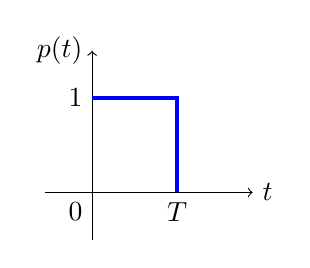
\begin{tikzpicture}[scale=1.2]
    
    \draw[->] (0,-0.5) -- (0,1.5) node[left] {$p(t)$};
    \draw[->] (-0.5,0) -- (1.7,0) node[below,right] {$t$};
    
    \draw[very thick, blue] (0,1) -- ++(0.9,0) -- ++(0,-1);
    
    \draw (0.9,0) node[below] {$T$};
    \draw (0,0) node[below left] {$0$};
    \draw (0,1) node[left] {$1$};
    
    \end{tikzpicture}
    
    \begin{align*}
    p(t) &= \mathrm u(t) - \mathrm{u}(t-T) \\
    \mathscr L \left\lbrace p(t) \right\rbrace &=
    \mathscr L \left\lbrace \mathrm u(t) \right\rbrace
    - \mathscr L \left\lbrace \mathrm{u}(t-T) \right\rbrace
    \\ &= \frac{1}{s} - \frac{1}{s} e^{-sT} = \frac{1-e^{-sT}}{s}
    \end{align*}
    
    \paragraph{Ex. 2}
    \mbox{}
    
    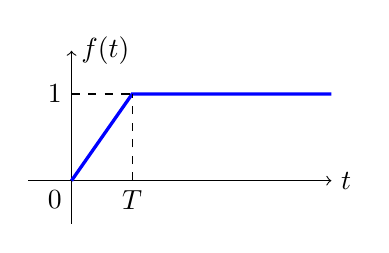
\begin{tikzpicture}[scale=1.1]
    
    \draw[->] (0,-0.5) -- (0,1.5) node[right] {$f(t)$};
    \draw[->] (-0.5,0) -- (3,0) node[below,right] {$t$};
    
    \draw[very thick, blue] (0,0) -- (0.7,1) -- (3,1);
    
    \draw[dashed] (0.7,0) node[below] {$T$} -- ++(0,1);
    \draw (0,0) node[below left] {$0$};
    \draw[dashed] (0,1) node[left] {$1$} -- ++(0.7,0);
    
    \end{tikzpicture}
    
    \begin{align*}
    f(t) &= \frac{t}{T}\mathrm u(t) - \frac{t-T}{T}\mathrm u(t-T) \\
    F(s) &= \frac{1}{T}\frac{1}{s^2} - \frac{1}{T}\frac{1}{s^2}e^{-sT}
    \\ &= \frac{1}{Ts^2}\left[ 1-e^{-sT} \right],\quad s>0 
    \end{align*}
    
    \paragraph{Ex. 3}
    \mbox{} \\
    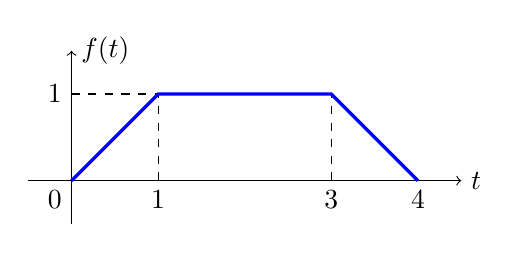
\begin{tikzpicture}[scale=1.1]
    
    \draw[->] (0,-0.5) -- (0,1.5) node[right] {$f(t)$};
    \draw[->] (-0.5,0) -- (4.5,0) node[below,right] {$t$};
    
    \draw[dashed] (1,0) node[below] {$1$} -- ++(0,1);
    \draw (0,0) node[below left] {$0$};
    \draw[dashed] (0,1) node[left] {$1$} -- ++(1,0);
    \draw[dashed] (3,0) node[below] {$3$} -- ++(0,1);
    \draw (4,0) node[below] {$4$};
    
    \draw[very thick, blue] (0,0) -- (1,1) -- (3,1) -- (4,0);
    
    \end{tikzpicture}
    
    \begin{align*}
    f(t) &= t\mathrm u(t) - (t-1)\mathrm u(t-1) - (t-3)\mathrm u(t-3)
    + (t-4)\mathrm u(t-4) \\
    F(s) &= \frac{1}{s^2} \left[
    1-e^{-s}-e^{-3s}+e^{-4s}
    \right]
    \end{align*}

    \paragraph{Ex. 4}
    \mbox{} \\
        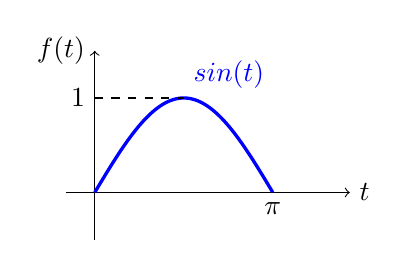
\begin{tikzpicture}[xscale=0.6,scale=1.2]
       
        \draw[->] (0,-0.5) -- (0,1.5) node[left] {$f(t)$};
        \draw[->] (-0.5,0) -- (4.5,0) node[below,right] {$t$};
        
        \draw[samples=200,domain=0:pi,smooth,variable=\x,blue,very thick] 
        plot ({\x},{sin(\x r)});
        
        \draw[dashed] (0,1) node[left] {$1$} -- (pi/2,1)
        node[above right,blue] {$\mathsmaller{sin(t)}$};
        \draw (pi,0) node[below] {$\pi$};
        \end{tikzpicture}
    \begin{align*}
    f(t) &= \sin(t)\mathrm u(t) + \sin(t-\pi)\mathrm u(t-\pi) \\
    F(s) &= \frac{1}{s^2}+\frac{1}{s^2+1}e^{-\pi s}
    \end{align*}
    
    \paragraph{Ex. 5}
    \mbox {} \\
        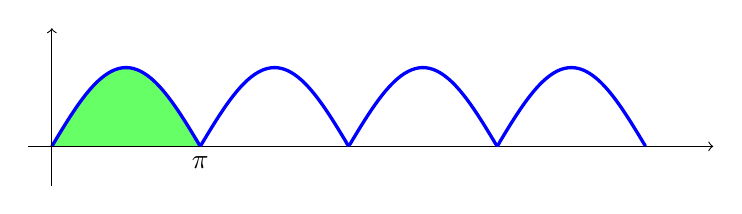
\begin{tikzpicture}[xscale=0.6]
        
        \filldraw
        [samples=200,domain=0:pi,smooth,variable=\x,blue,very thick,fill=green!60] 
        plot ({\x},{sin(\x r)});
        
        \draw[->] (0,-0.5) -- (0,1.5); %node[left] {$f(t)$};
        \draw[->] (-0.5,0) -- (14,0); %node[below,right] {$t$};
        
        \draw[samples=200,domain=pi:4*pi,smooth,variable=\x,blue,very thick] 
        plot ({\x},{abs(sin(\x r))});
        
        \draw (pi,0) node[below] {$\pi$};
        
        \end{tikzpicture}
    \begin{align*}
    f(t) &= |\sin t|\mathrm u(t) \\
    F(s) &= \frac{1+e^{-\pi s}}{1-e^{-\pi s}}
    \end{align*}
    
    \paragraph{Ex. 6}
    \begin{align*}
    F(s) = \underset{\text{αιτιατής συνάρτησης}}{\frac{s^2-6}{s^3+4s^2+3s}}
    = \frac{s^2 - 6}{s(s^2+4s+3)} &= \frac{s^2-6}{s(s+1)(s+3)}
    = \frac{A}{s} + \frac{B}{s+1} + \frac{\varGamma}{s+3}
    \\ &= \frac{-2}{s} + \frac{\sfrac{5}{2} }{s+1}+\frac{\sfrac{1}{2} }{s+3}
    \\ f(t) &= \left[ 
    -2+\frac{5}{2} e^{-t} + \frac{1}{2} e^{-3t}
    \right]\mathrm u(t)
    \end{align*}
    
    \paragraph{Ex. 7}
    \begin{align*}
    F(s) &= \frac{5s^3-6s-3}{s^3(s+1)^2} =
    \frac{A}{s} + \frac{B}{s^2} + \frac{\varGamma}{s^3}
    + \frac{\varDelta}{(s+1)} + \frac{E}{(s+1)^2} \\
    F(s) &= \frac{-3}{s} - \frac{3}{s^3} - \frac{3}{s+1} + \frac{2}{(s+1)^2}
    \\ f(t) &= \left[-3 - \frac{3}{2} t^2 - 3e^{-t} + 2te^{-t} \right] \mathrm u(t)
    \end{align*}
    
    \paragraph{Ex. 8}
    \begin{align*}
    F(s) = \frac{16}{s(s^2+4)^2} &=
    \frac{A}{s} + \frac{B_1s + C_1}{s^2+4} + \frac{B_2s+C_2}{(s^2+4)^2} \\
    16 &= A(s^2+4)^2 + (B_1s+C_1)s(s^2+4) + (B_2s+C_2)s \\
    F(s) &= \frac{1}{s} - \frac{s}{s^2+4} - \frac{4s}{(s^2+4)^2} \\
    f(t) &= \left[ 1-\cos 2t - t\sin 2t \right] \mathrm u(t)
    \end{align*}
    
    \paragraph{Ex. 9}
    \[
    f''' + 6f'' + 11f' + 6f = 1 \qquad t\geq 0 \qquad
    \underbrace{f=f'=f''}_{@ 0^-}=0
    \]
    \begin{align*}
    \mathscr{LT}\left\lbrace \qquad \right\rbrace & \\
    s^3F - \cancel{s^2f_0 - sf_0' -f_0''}
    +6 \left[ s^2F-\cancel{sf_0-f_0} \right]
     + 11 \left[ sF - \cancel{f_0} \right] + 6F
    &= \frac{1}{s} \\
    F(s^3+6s^2+11s+6)&= \frac{1}{s}
    \implies F(s) = \frac{1}{s(s+1)(s+2)(s+3)}
    \\ F(s) &= \frac{\sfrac{1}{6} }{s}
    + \frac{-\sfrac{1}{2} }{s+1}
    + \frac{\sfrac{1}{2} }{s+1}
    + \frac{-\sfrac{1}{6} }{s+3} \\
    f(t) &= \left[
    \frac{1}{6}-\frac{1}{2}e^{-t}+\frac{1}{2}e^{-2t}-\frac{1}{6}e^{-3t}
    \right]\mathrm u(t)
    \end{align*}
    
    Η μόνιμη κατάσταση που συντηρείται από το 1 στην διαφορική εξίσωση είναι το
    \( \frac{1}{6} \)
